% Final English edition. Same model and results as paper.tex.
\documentclass[11pt]{article}
\usepackage[utf8]{inputenc}
\usepackage[T1]{fontenc}
\usepackage[english]{babel}
\usepackage[margin=1in]{geometry}
\usepackage{amsmath,amssymb,amsthm,booktabs,array,longtable,graphicx}
\usepackage[round]{natbib}
\usepackage[colorlinks=true,allcolors=blue!50!black]{hyperref}
\usepackage{xcolor}
\newtheorem{proposition}{Proposition}
\theoremstyle{definition}\newtheorem{assumption}{Assumption}
\newcolumntype{L}[1]{>{\raggedright\arraybackslash}p{#1}}
\newcommand{\R}{\mathbb R}
\newcommand{\E}{\mathbb E}
\newcommand{\threshold}{0.640}
\newcommand{\betaZero}{0.130}
\newcommand{\betaOne}{-0.085}
\newcommand{\riskMin}{8.89}
\newcommand{\riskMax}{23.80}
\newcommand{\effortMin}{0.224}
\newcommand{\effortMax}{0.400}
\newcommand{\cohortSlope}{0.130}
\newcommand{\stockSlope}{-0.034}

\title{Relative Loan Pricing as a Signal of Delinquency:\\
\large Credit Screening, Constraints, and Portfolio Composition}
\author{Fabián Matías Galarza Chumbe\thanks{Universidad del Pacífico.
Final project for AI and Economic Modeling, Track B. This article develops
the theoretical foundation of the research on relative loan pricing and
delinquency initiated with William Brandon Grados Taco. Replication materials:
\url{https://github.com/fgalarzac/ai-project}. The appendix documents
collaboration with artificial intelligence.}}
\date{November 24, 2026}
\begin{document}
\maketitle
\begin{abstract}
New-loan prices are observed before loan performance and can therefore
inform bank supervision. Their relationship with subsequent delinquency,
however, depends on mechanisms that operate in opposite directions. This
article solves a bank's screening decision conditional on its loan rate
relative to other banks. With linear adverse selection and a quadratic
screening cost, the risk slope is $a-g^2/c$ only at an interior solution:
$a$ captures applicant selection and $g^2/c$ the screening response.
Limited capacity and the probability floor change that slope. A sign reversal
across opacity segments requires explicit crossing and interiority conditions.
When new and old loans are aggregated, portfolio composition can reverse the
sign of origination risk. Three propositions, complete proofs, and symbolic
and numerical checks establish these conditions. The results provide an
interpretation of the indicator for Peruvian banking; the simulations are
illustrative and do not constitute a predictive estimation exercise.
\end{abstract}

\section{Introduction}
A loan's price is known at origination, whereas its credit performance is
revealed later. This timing difference makes it relevant to ask whether an
unusually high rate relative to comparable banks can anticipate delinquency.
For a supervisor, such a signal can help direct scrutiny towards a bank
before deterioration becomes visible on its balance sheet. The question is
particularly important when available data combine rates on recent lending
with quality indicators for a portfolio containing loans of different ages.

The sign of the relationship is not immediate. A higher rate may attract
riskier applicants, but it also increases the benefit of avoiding a delinquent
loan and thus the bank's incentive to screen. A reduction in new lending
also changes its weight in the total outstanding balance. If new loans are
riskier than the legacy portfolio, their smaller share can lower aggregate
delinquency even as their individual risk increases. Selection, screening,
and composition are therefore distinct mechanisms that must be separated
when interpreting relative loan pricing.

This article develops an economic model of that interpretation for the
Peruvian banking question. The bank chooses how intensively to screen a loan,
given its price and the segment's technology. Adverse selection increases
pre-screening risk with price; screening reduces it at an increasing cost.
Two constraints bound effort: operational capacity and the impossibility of
a negative probability. Solving the problem under both constraints identifies
when effort responds and when only applicant quality changes.

The first result characterises a unique maximum and distinguishes three
regimes. At an interior solution, selection dominates if $a>g^2/c$, where
$a$ measures the sensitivity of pre-screening risk to price, $g$ screening
productivity, and $c$ the scale of its quadratic cost. When capacity is
exhausted, effort stops responding and the risk slope is $a$. At the
probability floor, that slope is zero. The second result establishes a
unique opacity threshold under continuity, strict decrease, crossing, and
interiority conditions. The third derives transmission to the portfolio
ratio and an exact condition under which composition reverses the sign.

The closest empirical antecedent is \citet{morgan2003}, who find information
about subsequent performance in rates on newly extended commercial and
industrial loans. The contribution here is to specify the conditions for
interpreting such a signal when screening is endogenous and the observed
outcome is an outstanding-balance ratio. The global solution and the
composition identity bring together familiar ingredients in an explicit
banking problem. The analysis is theoretical and conditional on price;
its predictive application to Peru requires a separate empirical assessment.

The exposition follows the mechanism. Proposition~\ref{p:global} solves
the effort decision. Proposition~\ref{p:threshold} compares segments with
different opacity at the same price. Proposition~\ref{p:stock} aggregates
the resulting risk with a legacy portfolio. Simulations examine the
conditions and failure cases of each result; the discussion draws out
their implications for measurement and forecasting.

\section{Institutional Evidence and Measurement}
\subsection{Lending rates and portfolio indicators}
The Peruvian banking supervisor, SBS, publishes effective annual rates by
institution and transaction type. Section 3 of its methodology defines
averages for transactions over the preceding thirty business days, weighted
by amounts disbursed \citep{sbsmetodo}. These are rates on \emph{flows}:
they describe recent loans and differ from rates on outstanding balances.
Because thirty-business-day windows can overlap across month-end observations,
they are not exact calendar-month cohorts either. Grouping by transaction
type, maturity, and currency improves comparability, although collateral,
borrower quality, and lending relationships may still differ.

Peruvian evidence illustrates why these distinctions matter.
\citet{choy2015} document the role of operating costs and risk in rate
differences across segments during 2010--2014. A high rate can reflect these
components as well as adverse selection. Moreover, overdue loans, loans more
than ninety days past due, and the high-risk portfolio measure (CAR, its
Spanish acronym) refer to different credit events. Linking a rate to a
probability requires specifying the event, population, and observation horizon.

The Central Reserve Bank of Peru (BCRP), in its November 2024 Financial
Stability Report, presents both
outstanding-balance indicators and vintage tracking in Table 2.2 and
Figure 2.7 \citep{bcrp2024}. Figure~\ref{fig:context} reproduces four series
from the table and shows persistent differences across segments. Adjusted
CAR includes write-offs over the preceding twelve months and covers the
financial system, a broader population than commercial banks. It retains
that definition here as institutional context, rather than as a calibration
target or a substitute for the thesis outcome variable.

\begin{figure}[htbp]
\centering
\begin{minipage}{.96\linewidth}
\centering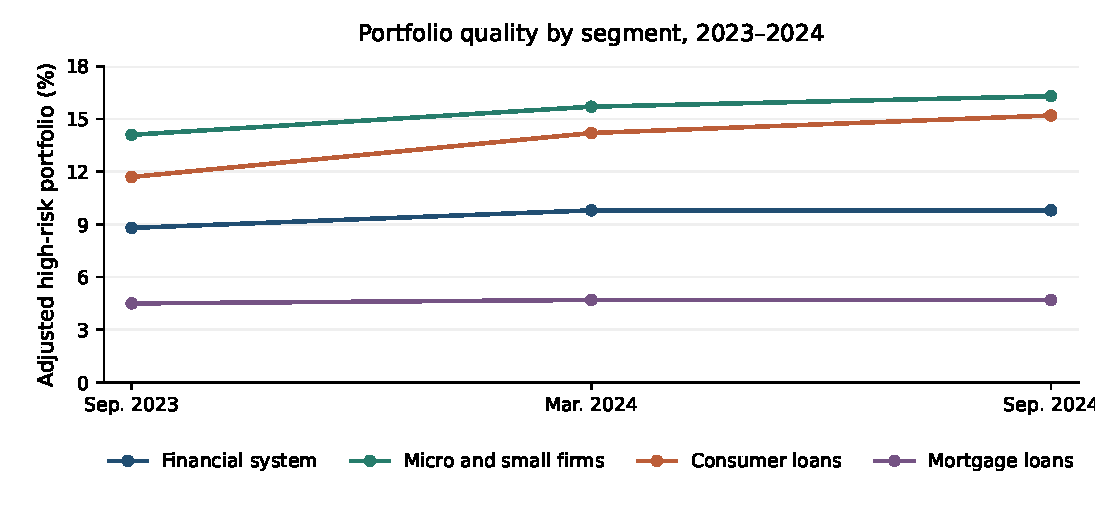
\includegraphics[width=\linewidth]{../code/figures/public_context_en.pdf}
\caption{Portfolio quality by segment. High-risk portfolio adjusted for
write-offs over the preceding twelve months, in per cent; financial system.
Source: BCRP, Financial Stability Report,
November 2024, Table 2.2, p. 21. The reproducible transcription is in
\texttt{code/data/}.}\label{fig:context}
\end{minipage}
\end{figure}

The article's quantitative analysis consists of model simulations and this
limited transcription of public statistics. Simulation parameters are
hypothetical. The economic interpretation of the results is distinct from
parameter estimation or forecast evaluation.

\subsection{Definition of the relative loan rate}
Let $j$ index banks, $s$ a cell defined by credit type, transaction type or
maturity band, and currency, and $t$ the reporting date. Write $i_{jst}$ for
the annual rate in decimals and $b_{st}$ for a common base in the same
currency. Let $\mathcal P_{-j,st}$ be the set of other banks with valid
observations and $n_{-j,st}$ its size. The relative loan rate is
\begin{equation}\label{eq:D}
D_{jst}=(i_{jst}-b_{st})-
\frac{1}{n_{-j,st}}\sum_{k\in\mathcal P_{-j,st}}(i_{kst}-b_{st})
=i_{jst}-\frac{1}{n_{-j,st}}\sum_k i_{kst}.
\end{equation}
The bank being evaluated is excluded from its reference group. A value
$D=0.02$ means a rate two percentage points above the peer average. The
simple mean provides a transparent comparison when disbursements by band
are unobserved; it differs from a transaction-weighted system rate. An
empirical application must fix comparability rules and require at least
three valid peers before evaluating predictive performance.

The median provides a sensitivity measure. It reduces the influence of
extreme rates but changes the comparator and may even change the gap's sign.
With hypothetical peer rates of 8, 9, 10, and 25\%, an own rate of 12\% is
one percentage point below the mean and 2.5 points above the median. Both
differences are checked in the code. The comparator must be chosen before
forecast errors are evaluated.

Cancellation of the common base in \eqref{eq:D} is algebraic. It does not
remove heterogeneous exposures to the same shock. If
$i_j=b+\lambda_j z+v_j$, where $z$ is the aggregate shock, $\lambda_j$ the
bank's exposure, and $v_j$ its specific component, the peer difference retains
$(\lambda_j-\bar\lambda_{-j})z+(v_j-\bar v_{-j})$. Bars denote averages over
other banks. Funding, costs, clientele, and margins can therefore continue
to affect the gap. A change in the peer set can also move $D$ while the
bank's own rate remains unchanged. Relative comparison improves the
description of price but is not a causal identification strategy.

\section{Related Literature and Mechanisms}
\citet{morgan2003} find predictive content in rates on new US commercial
and industrial loans for subsequent performance and supervisory ratings.
Their published 2003 finding motivates the informational use of prices.
The present analysis examines an additional distinction: new-cohort quality
and the outstanding-balance ratio of a portfolio may respond differently.
The US evidence does not by itself establish the sign of that relationship
for Peruvian banks.

The selection mechanism relates to \citet{stiglitz1981}, p. 393: price
changes the composition and incentives of credit applicants. The model
summarises the first channel with a positive sensitivity of pre-screening
risk to price. \citet{broecker1990} studies imperfect tests and interbank
competition; \citet{ruckes2004} relates credit standards and competition to
economic prospects; and \citet{dellariccia2006} distinguishes screening and
pooling regimes. These published articles provide the theoretical context.
The contribution focuses on a screening decision conditional on price and
its connection to portfolio composition.

For Peruvian measurement, \citet{yamunaque2024} constructs a measure of
deterioration among initially performing loans over twelve months and
distinguishes it from the accounting delinquency ratio. The reference is
cited as BCRP Working Paper 2024-015, the editorial status verified in its
catalogue. This distinction supports an explicit choice of event and horizon:
a probability of deterioration cannot automatically be equated with any
published delinquency series. \citet{clark2007} develops a comparison of
nested forecasting models relevant to a subsequent evaluation of the
incremental information in relative loan pricing.

The mechanisms imply different observable patterns. When selection
dominates, higher prices accompany poorer new-vintage quality, holding
screening fixed. When screening dominates, a higher price must be accompanied
by an effective effort response and lower subsequent risk, provided capacity
allows that response. When composition dominates, the sign changes upon
aggregation and depends on cohort weights. Distinguishing these patterns
requires information on vintages, balances, screening, and collateral;
average rates alone do not identify which mechanism is operating.

\section{Model}\label{sec:model}
\subsection{Agents, information, units, and timing}
The only optimising agent is a risk-neutral bank. Applicants and peer banks
determine a reduced-form risk pool and reference rate; their strategic game
is not modelled. The supervisor observes $D$ and subsequently a portfolio
ratio, but neither effort nor the full risk composition. Opacity
$\kappa\in[0,1]$ is an exogenous segment characteristic: a larger value means
less initially verifiable information. It organises the theoretical comparison
and is not automatically identified with an observed category such as small firms.

The timing is as follows. Segment, technology, and observed price are fixed
first; the applicant pool then forms and its mean risk is observed by the bank.
The bank chooses screening effort before origination. Finally, credit outcomes
are realised and the portfolio is observed at horizon $h$. The bank knows the
parameters when choosing effort. Performance uncertainty remains and is
integrated into its objective. Price is an argument of this continuation
problem, rather than a variable determined in equilibrium.

The objects $q^0$ and $q$ are dimensionless probabilities for the same event
and horizon in a standardised cohort. Effort $e$ and opacity $\kappa$ are
indices. The relative rate $D$ is measured in annual decimal-rate units.
Payoffs and costs are normalised per unit of lending. The sensitivity of the
performance payoff to one unit of $D$ is normalised to one. This is a payoff
simplification, not an exact conversion of effective rates across arbitrary
contractual maturities.

Three operations must be distinguished. In choosing $e$, the bank holds
$D$ and $\kappa$ fixed and compares effort levels at the same price and
segment. In calculating $\partial_Dq^*$, it compares nearby prices within
the same technology and allows effort to adjust optimally. Only
Proposition~\ref{p:threshold} compares different values of $\kappa$, always
at the same price $D_0$. A prime on $M$ denotes a derivative with respect
to $D$; primes on $g$ and $c$ in the opacity analysis refer to $\kappa$.

The table collects notation and units. Portfolio objects enter only in
Proposition~\ref{p:stock}; they do not affect the initial effort choice.
\begin{center}\small
\begin{tabular}{@{}L{.15\linewidth}L{.51\linewidth}L{.27\linewidth}@{}}
\toprule Symbol & Meaning & Unit or restriction\\\midrule
$D$ & Own rate minus the simple peer mean & Annual decimal rate\\
$\kappa$ & Exogenous segment opacity & Index in $[0,1]$\\
$\bar q,a$ & Reference risk and selection sensitivity & Probability; $a>0$\\
$q^0,q,q^*$ & Pre-screening, screened, and optimal risk & Same event and horizon\\
$e,\bar e,u$ & Effort, capacity, and maximum feasible effort & Nonnegative indices\\
$g,c$ & Screening productivity and cost scale & Both positive\\
$R,\bar R,F$ & Performance payoff, reference payoff, and fixed cost & Per unit of lending\\
$z$ & Unconstrained desired effort: $gR/c$ & Effort index\\
$H,\beta$ & Screening strength $g^2/c$ and net slope $a-H$ & Risk per unit of $D$\\
$\beta_D$ & Derivative of $q^*$ in the effective regime & Risk per unit of $D$\\
$B_0,B,B_1$ & Legacy, new, and new-at-$D=0$ balances & Same monetary unit\\
$m_0,w,M$ & Legacy delinquency, new weight, and total ratio & Fractions in $[0,1]$\\
$\varepsilon$ & Proportional sensitivity of $B$ to price & Per unit of $D$\\
\bottomrule
\end{tabular}
\end{center}

\begin{assumption}[Selection and domain]\label{as:selection}
For each fixed $\kappa$, $a=a(\kappa)>0$, $\bar q\in(0,1)$, and $D$ belongs
to a compact interval $\mathcal D$. Pre-screening risk is
$q^0(D,\kappa)=\bar q+a(\kappa)D\in[0,1]$ throughout $\mathcal D$.
\end{assumption}
The affine form is a local approximation to changes in the applicant pool.
A one-percentage-point rate increase means $\Delta D=0.01$ and changes risk
by $0.01a$ probability units, or $a$ percentage points. For example, with
$a=0.18$, the change is $0.0018$, equivalent to $0.18$ percentage points.
The approximation is restricted to the admissible domain. Its positive slope
represents adverse selection, rather than an empirical universal or a response
derived from an explicit optimisation problem for each borrower.

The probability restriction also bounds comparable prices. Subtracting
$\bar q$ and dividing by $a>0$ gives
\[
0\le\bar q+aD\le1
\quad\Longleftrightarrow\quad
-\frac{\bar q}{a}\le D\le\frac{1-\bar q}{a}.
\]
The compact domain $\mathcal D$ lies within this interval and must also
satisfy the positive-payoff condition in Assumption~\ref{as:payoff}.
An affine probability is not extrapolated to arbitrary loan rates.

\begin{assumption}[Technology, capacity, and cost]\label{as:technology}
$g=g(\kappa)>0$, $c=c(\kappa)>0$, and $\bar e\ge0$ are finite. For a
normalised loan volume, $q(D,e,\kappa)=q^0(D,\kappa)-g(\kappa)e$ and the
screening cost is $c(\kappa)e^2/2$. Feasible effort satisfies
\[
0\le e\le u(D,\kappa):=\min\{\bar e,q^0(D,\kappa)/g(\kappa)\}.
\]
\end{assumption}
The bound $q^0/g$ prevents negative probabilities. Capacity $\bar e$ can
represent screening staff or time. Screening includes verification and
contractual conditions that reduce the risk of originated loans. Volume is
held fixed with respect to effort: the model abstracts from endogenous
rejection composition and replacement costs. If screening removes applicants
without replacement, volume depends on $e$ and the solution changes. The
linear technology can reach zero risk, a mathematical boundary of limited
realism rather than a feasible supervisory target.

The second effort bound follows directly from $q\ge0$: since $g>0$,
$q^0-ge\ge0$ is equivalent to $e\le q^0/g$. The first bound,
$e\le\bar e$, is technological. Satisfying both requires their minimum.
Moreover, $e\ge0$ ensures $q\le q^0\le1$. Thus $0\le e\le u$ rules out
negative effort and negative risk while respecting capacity.

\begin{assumption}[Payoff and conditional problem]\label{as:payoff}
The normalised performance payoff is $R(D)=\bar R+D>0$, and $F$ is a
per-unit cost independent of $e$. The bank solves
\begin{equation}\label{eq:problem}
\max_{e\in[0,u(D,\kappa)]}\pi(e;D,\kappa)
=[1-q^0(D,\kappa)+g(\kappa)e]R(D)-F-\frac{c(\kappa)}2e^2.
\end{equation}
Price, the peer reference, and $\kappa$ are held fixed when comparing
deviations in effort.
\end{assumption}
Fixed cost $F$ does not affect optimal effort. Nor does a strictly positive
volume multiplying the entire objective, provided it is independent of $e$.
The participation decision is outside the problem: the result concerns a
unit of credit the bank is already considering originating. The payoff assumes
that avoiding the adverse event improves expected receipts. Recoveries,
insurance, or collateral that vary with price or effort would require a
different payoff. The event horizon and contractual cash flow must also be
compatible in an empirical implementation.

To interpret the objective, start with $1-q^0+ge=1-q$, the probability of
avoiding the adverse event. Multiplying it by $R$ gives the expected payoff;
fixed and screening costs are then deducted. An additional unit of effort
produces marginal benefit $gR$ at marginal cost $ce$. A higher price increases
$R$, whereas greater effort raises marginal cost. This comparison explains
the bank's response but does not yet establish whether desired effort fits
within the constraints.

\section{Results and Complete Proofs}
\subsection{Optimal screening under all constraints}
\begin{proposition}[Global solution and regime-specific slopes]\label{p:global}
Under Assumptions~\ref{as:selection}--\ref{as:payoff}, problem
\eqref{eq:problem} has a unique maximum. It is
\begin{equation}\label{eq:opt}
e^*=\min\left\{\frac{gR(D)}c,\bar e,\frac{q^0(D)}g\right\},\qquad
q^*=\max\left\{0,q^0(D)-g\min\left\{\bar e,\frac{gR(D)}c\right\}\right\}.
\end{equation}
For fixed $\kappa$, on any open interval with strict inequalities maintaining
the regime, the slopes are
\begin{equation}\label{eq:regimes}
\frac{\partial q^*}{\partial D}=
\begin{cases}
a-g^2/c,&gR/c<\bar e\ \text{and}\ gR/c<q^0/g,\\
a,&\bar e<gR/c\ \text{and}\ \bar e<q^0/g,\\
0,&q^0/g<gR/c\ \text{and}\ q^0/g<\bar e.
\end{cases}
\end{equation}
If $\bar e=0$, then $e^*=0$ and $q^*=q^0$, with slope $a$ in the interior
of the price domain. At ties between constraints, the solution is continuous
and one-sided derivatives apply; an ordinary derivative need not exist.
\end{proposition}
\begin{proof}
\textbf{Step 1: feasibility, existence, and uniqueness.}\par
Fix $D$ and $\kappa$, so $q^0,R,g,c,\bar e$ are constant when comparing
effort. Since $q^0\ge0$, $g>0$, and $\bar e\ge0$, the upper bound satisfies
$u\ge0$. The interval $[0,u]$ is nonempty and compact and $\pi$ is
continuous, so the extreme value theorem gives a maximum. If $u=0$, the
only choice is $e=0$. If $u>0$, the second derivative is $\pi_{ee}=-c<0$;
strict concavity on a convex interval rules out two distinct maximisers.

\textbf{Step 2: first order identifies desired effort.}\par
Differentiating with respect to $e$, holding price and segment fixed, gives
\[
\pi_e=gR-ce,\qquad \pi_e=0\ \Longleftrightarrow\ e=z:=gR/c>0.
\]
Equality of marginal benefit and marginal cost does not establish $z\le u$.
Thus $z$ is still an unconstrained candidate.

\textbf{Step 3: solve the constrained problem.}\par
Completing the square shows how to proceed if that candidate is infeasible:
\begin{align*}
gRe-\frac c2e^2
 &=-\frac c2\left[e^2-2\frac{gR}{c}e\right]
  =-\frac c2\left[(e-z)^2-z^2\right],\\
\pi(e)&=\underbrace{(1-q^0)R-F+\frac{(gR)^2}{2c}}_{\text{constant with respect to }e}
              -\frac c2(e-z)^2.
\end{align*}
Since $c>0$, maximising $\pi$ is equivalent to minimising $(e-z)^2$ on
$[0,u]$. If $z\le u$, the unique point at zero distance is $e=z$.
If $z>u$, every $e<u$ satisfies $z-e>z-u>0$, so squaring gives
$(e-z)^2>(u-z)^2$. The unique maximum is then $e=u$. This also includes
$u=0$; if $z=u$, both arguments identify the same point. Consequently,
\[
e^*=\min\{z,u\}=\min\{gR/c,\bar e,q^0/g\}.
\]

\textbf{Step 4: substitute into risk and verify its bounds.}\par
Define $v=\min\{\bar e,gR/c\}\ge0$. If $v\le q^0/g$, then $e^*=v$ and
$q^*=q^0-gv\ge0$. If $v>q^0/g$, then $e^*=q^0/g$ and $q^*=0$.
These cases are exactly $q^*=\max\{0,q^0-gv\}$. Moreover, $e^*\ge0$ and
$g>0$ imply $q^*\le q^0\le1$. This yields the second formula and verifies
that the result is a valid probability.

\textbf{Step 5: differentiate within each regime.}\par
With $\kappa$ fixed, strict inequalities persist in a neighbourhood of the
price under consideration. The locally active expression can be differentiated:
\begin{align*}
\text{Interior: }q^*&=\bar q+aD-\frac{g^2}{c}(\bar R+D),
 &\partial_Dq^*&=a-g^2/c;\\
\text{Capacity: }q^*&=\bar q+aD-g\bar e,
 &\partial_Dq^*&=a;\\
\text{Floor: }q^*&=0,
 &\partial_Dq^*&=0.
\end{align*}
At an interior solution, $\partial_De^*=g/c$: multiplying by productivity
$g$ gives the marginal risk reduction $g^2/c$. When capacity is exhausted,
effort no longer responds. At the floor, risk cannot decline further.

\textbf{Step 6: zero capacity and ties.}\par
If $\bar e=0$, the feasible set is $\{0\}$, giving $e^*=0$ and $q^*=q^0$;
its derivative inside the domain is $a$. For general capacity, the affine
functions entering the minimum are continuous. The minimum and maximum of
finitely many continuous functions are continuous, so neither $e^*$ nor
$q^*$ jumps. Both are also piecewise affine. Each side of a tie activates
one of these expressions, yielding one-sided slopes. If two expressions
coincide on an interval, their slopes are equal and no additional issue
arises. If the two slopes differ, the ordinary derivative does not exist;
the capacity example in Section~\ref{sec:sim} exhibits this case.
\end{proof}

The interpretation of $g^2/c$ has two steps: a higher price raises interior
effort by $g/c$, and each unit of effort reduces risk by $g$. Once capacity
is exhausted, the first response disappears. A bank with high screening
productivity can therefore have a positive risk slope when capacity is scarce.
The inequality $g^2/c>a$ alone is not a global sufficient condition.

\paragraph{A numerical walkthrough.}
The decision can be followed using the hypothetical simulation parameters:
$\bar q=0.28$, $a=0.18$, $g=\sqrt{0.05}$, $c=1$, $\bar R=1.10$, and
$\bar e=0.50$. At $D=0$, $q^0=0.28$ and $R=1.10$. Desired effort is
$gR/c\simeq0.246$, below capacity $0.50$ and the probability bound
$q^0/g\simeq1.252$, so the bank is interior. Screening reduces risk by
$ge^*=0.055$, leaving $q^*=0.225$. Locally, a one-percentage-point rate
increase adds $0.18$ percentage points through selection and subtracts
$0.05$ through screening, for a net $0.13$ percentage points. This illustrates
units and the mechanism; the values are not calibrated to Peruvian data.

\subsection{Conditions for an opacity threshold}
Define $H(\kappa)=g(\kappa)^2/c(\kappa)$ and
$\beta(\kappa)=a(\kappa)-H(\kappa)$.
\begin{assumption}[Sufficient crossing conditions]\label{as:cross}
On $\kappa\in[0,1]$, $a,g,c$ are continuous and positive. The function
$a-H$ is strictly decreasing and satisfies $a(0)>H(0)$ and $a(1)<H(1)$.
At the common comparison price $D_0$, both interiority inequalities in the
first line of \eqref{eq:regimes} hold strictly for every $\kappa$.
\end{assumption}
\begin{proposition}[Conditional threshold]\label{p:threshold}
Under Assumptions~\ref{as:selection}--\ref{as:cross}, there is a unique
$\kappa^*\in(0,1)$ such that $\partial_Dq^*(D_0,\kappa^*)=0$. The
derivative is positive for $\kappa<\kappa^*$ and negative for $\kappa>\kappa^*$.
\end{proposition}
\begin{proof}
\textbf{Step 1: continuity of the net slope.}\par
By S4, $a,g,c$ are continuous on $[0,1]$ and $c$ is strictly positive.
Squaring and division preserve continuity when the denominator does not
vanish. Thus $H=g^2/c$ and $\beta=a-H$ are continuous.

\textbf{Step 2: existence of an interior zero.}\par
S4 implies $\beta(0)=a(0)-H(0)>0$ and $\beta(1)=a(1)-H(1)<0$. The
intermediate value theorem gives $\kappa^*\in(0,1)$ with
$\beta(\kappa^*)=0$. The zero is interior because neither endpoint is zero.

\textbf{Step 3: uniqueness and signs on either side.}\par
If $x<y$ were two zeros, strict decrease would give
$0=\beta(x)>\beta(y)=0$, a contradiction. For any $\kappa<\kappa^*$,
the same property gives $\beta(\kappa)>\beta(\kappa^*)=0$; for
$\kappa>\kappa^*$, it gives the reverse inequality. Hence the zero is
unique and the signs are ordered as stated.

\textbf{Step 4: return to the risk derivative.}\par
The zero established so far concerns a function of primitives. Its economic
interpretation uses the final part of S4: at the common price $D_0$, effort
is interior for every $\kappa$. The first line of \eqref{eq:regimes} gives
$\partial_Dq^*(D_0,\kappa)=a(\kappa)-g(\kappa)^2/c(\kappa)=\beta(\kappa)$.
The unique zero and signs are therefore precisely those in the proposition.
Without interiority, the zero of $\beta$ would not characterise the slope
in the effective regime.
\end{proof}

Assumption~\ref{as:cross} is a testable economic restriction, rather than
the definition of opacity. When the functions are differentiable,
\begin{equation}\label{eq:logs}
\frac{H'}H=2\frac{g'}g-\frac{c'}c.
\end{equation}
Limited initial information might leave greater scope for further
verification, but this does not establish $g'>0$. If information is harder
to obtain, $g'\le0$ and $c'\ge0$ are plausible, giving $H'\le0$.
Crossing may fail, or may still occur if $a$ falls sufficiently quickly.
Thus $H'>0$ alone is not necessary, and continuity alone does not ensure
uniqueness. A stronger sufficient criterion is $a'<0$, $H'>0$, and endpoint
crossing. The proposition only requires that $a-H$ strictly decrease.
The sensitivity analysis explicitly considers a technology that deteriorates
with opacity.

\subsection{From a new cohort to the portfolio balance}
Fix horizon $h$. Let $B_0>0$ be the outstanding legacy balance at that date
and $m_0\in[0,1]$ its fraction in the chosen delinquency state. Let $B(D)>0$
be the balance of the new cohort remaining at $h$ after normal amortisation.
Define $w(D)=B(D)/(B_0+B(D))$.

A balance example clarifies the weight before differentiation. With legacy
balance four and new balance one, the new weight is $1/(4+1)=0.20$: eighty
per cent of the ratio corresponds to old loans. A change in new-loan quality
therefore does not change the same fraction of the total portfolio. Its
effect also depends on the cohort's weight.

\begin{assumption}[Accounting and seasoning]\label{as:stock}
At the horizon, each cohort balance is deterministic or interpreted as the
exposure of a continuum population. Risk $q^*(D)$ equals the expected fraction
of its balance in the chosen credit event, conditional on remaining in the
portfolio. Amortisation and loan size do not select additional risk beyond
that captured by $q^*$. The quantities $B_0,m_0$ are constant with respect to $D$;
$B(D)>0$ is differentiable. No write-offs, portfolio sales, or reclassifications
alter this identity in the exercise.
\end{assumption}
The compatibility required by this assumption is substantive. A lifetime
default probability is not the probability of being more than ninety days
past due on a specific date. Horizon, seasoning, persistence of delinquency,
and the remaining balance must be defined. If those processes vary with $D$,
they must enter $q^*$ or an expanded accounting framework.

\begin{proposition}[Transmission and composition]\label{p:stock}
Under Assumptions~\ref{as:selection}--\ref{as:payoff} and~\ref{as:stock},
the expected portfolio ratio is $M(D)=(1-w)m_0+wq^*(D)$. In any differentiable
regime, writing $\beta_D=\partial_Dq^*(D)$,
\begin{equation}\label{eq:stock}
M'(D)=w\beta_D+w'(q^*-m_0).
\end{equation}
If $B$ is constant, the sign is that of $\beta_D$. If $\beta_D\ne0$ and
$|w'(q^*-m_0)|<w|\beta_D|$, the sign is also preserved.
With $B(D)=B_1e^{-\varepsilon D}$, $B_1>0$, and $\varepsilon\ge0$,
\begin{equation}\label{eq:composition}
M'=w\{\beta_D-\varepsilon(1-w)(q^*-m_0)\}.
\end{equation}
In particular, if $\beta_D>0$ and $q^*>m_0$, then $M'<0$ if and only if
$\varepsilon(1-w)(q^*-m_0)>\beta_D$.
\end{proposition}
\begin{proof}
\textbf{Step 1: construct the ratio from comparable balances.}\par
Under S5, expected delinquent balance is $B_0m_0+Bq^*$. Its denominator
$B_0+B$ is deterministic and positive. Expected delinquent balance can
therefore be divided by that total; no unjustified interchange of an
expectation of ratios and a ratio of expectations is required. Separating
the two terms gives
\[
M=\frac{B_0}{B_0+B}m_0+\frac{B}{B_0+B}q^*
  =(1-w)m_0+wq^*,\qquad 0<w<1.
\]

\textbf{Step 2: identify quality and composition.}\par
Since $B_0,m_0$ are constant with respect to $D$, the product rule yields
\begin{align*}
M'&=-w'm_0+w'q^*+w\,\partial_Dq^*\\
  &=w\beta_D+w'(q^*-m_0),
\end{align*}
which is \eqref{eq:stock}. The first term changes new-loan quality holding
the weight fixed; the second changes the weight of a cohort whose quality
differs from that of the legacy portfolio.

\textbf{Step 3: verify the two sign-preservation rules.}\par
If $B$ is constant, $w$ is also constant, so $w'=0$ and $M'=w\beta_D$.
Because $w>0$, both have the same sign, including zero. For the second rule,
write $T=w'(q^*-m_0)$ for the composition term. If $\beta_D>0$ and
$|T|<w|\beta_D|=w\beta_D$, then
$M'=w\beta_D+T\ge w\beta_D-|T|>0$. If $\beta_D<0$, then
$w|\beta_D|=-w\beta_D$ and $M'\le w\beta_D+|T|<0$. The strict bound
prevents composition from cancelling or reversing the nonzero slope.

\textbf{Step 4: differentiate the cohort weight.}\par
The quotient rule, using $B_0'=0$, gives
\[
w'=\frac{B'(B_0+B)-BB'}{(B_0+B)^2}
   =\frac{B'B_0}{(B_0+B)^2}.
\]
For exponential balances, $B'=-\varepsilon B$. Substituting and using
$B/(B_0+B)=w$ and $B_0/(B_0+B)=1-w$ gives
$w'=-\varepsilon w(1-w)$. Inserting this into \eqref{eq:stock} yields
\eqref{eq:composition}.

\textbf{Step 5: obtain the exact reversal condition.}\par
Since $w>0$, the sign of $M'$ is the sign of the bracketed expression:
\[
M'<0\quad\Longleftrightarrow\quad
\beta_D-\varepsilon(1-w)(q^*-m_0)<0
\quad\Longleftrightarrow\quad
\varepsilon(1-w)(q^*-m_0)>\beta_D.
\]
With $\beta_D>0$ and $q^*>m_0$, this inequality describes a reversal:
new-loan risk worsens, but its weight in a safer legacy portfolio falls.
Equality gives a zero total slope, not a strict reversal. Every operation
is performed where $q^*$ is differentiable.
\end{proof}

The proposition captures dilution of a small cohort and a separate
composition mechanism: replacing safer legacy credit with riskier new loans.
When price rises and the new cohort loses weight, the total ratio can improve
while individual new-loan risk deteriorates. A predictive coefficient on an
outstanding-balance ratio therefore does not automatically distinguish
screening from composition. If $m_0$ varies with price, an additional term
$(1-w)m_0'$ appears; if $B_0$ changes, the specific formula for $w'$ also
changes. These exclusions have economic content.

In the exponential specification, $B_1$ is the new balance at $D=0$ and
$\varepsilon=-B'/B$ measures its proportional sensitivity to price. It is
a \emph{semi-elasticity} with respect to a decimal rate, rather than the
elasticity $DB'/B=-\varepsilon D$. If $\varepsilon=0$, balance is
unresponsive and the composition term disappears. If $\varepsilon>0$ and
$q^*>m_0$, a decline in the new weight reduces the total ratio; it dominates
only when the P3 threshold is exceeded.

\section{Simulations, Counterexamples, and Sensitivity}\label{sec:sim}
All parameters in this section are illustrative and are not fitted to Peru.
The interior scenario fixes $\bar q=0.28$, $\bar R=1.10$, $\bar e=0.50$,
and $D\in[-0.10,0.10]$, with
\[
a(\kappa)=0.18e^{-0.8\kappa},\quad
g(\kappa)=\sqrt{0.05}e^{0.8\kappa},\quad c(\kappa)=e^{0.4\kappa}.
\]
A ten-percentage-point range makes the mechanisms visible; it does not
represent typical observed variation. Fixed cost $F$ is normalised to zero
because it does not affect effort. The relatively high risk level displays
a broad feasible region rather than calibrating Peruvian delinquency.

\subsection{Conditional crossing and its failure}
In this scenario, $H=0.05e^{1.2\kappa}$ and
$\beta=0.18e^{-0.8\kappa}-0.05e^{1.2\kappa}$. Equating the two forces,
dividing by $0.05e^{-0.8\kappa}>0$, and taking logarithms gives
$\kappa^*=\log(3.6)/2=\threshold$. Endpoint slopes are \betaZero{} and
\betaOne{}. On a grid of 1001 opacity values and 121 prices, effort ranges
from \effortMin{} to \effortMax{}, and risk from \riskMin\% to \riskMax\%.
The code also checks feasibility at every point. These values are imported
from \texttt{code/output/numbers.tex}.

\begin{figure}[htbp]
\centering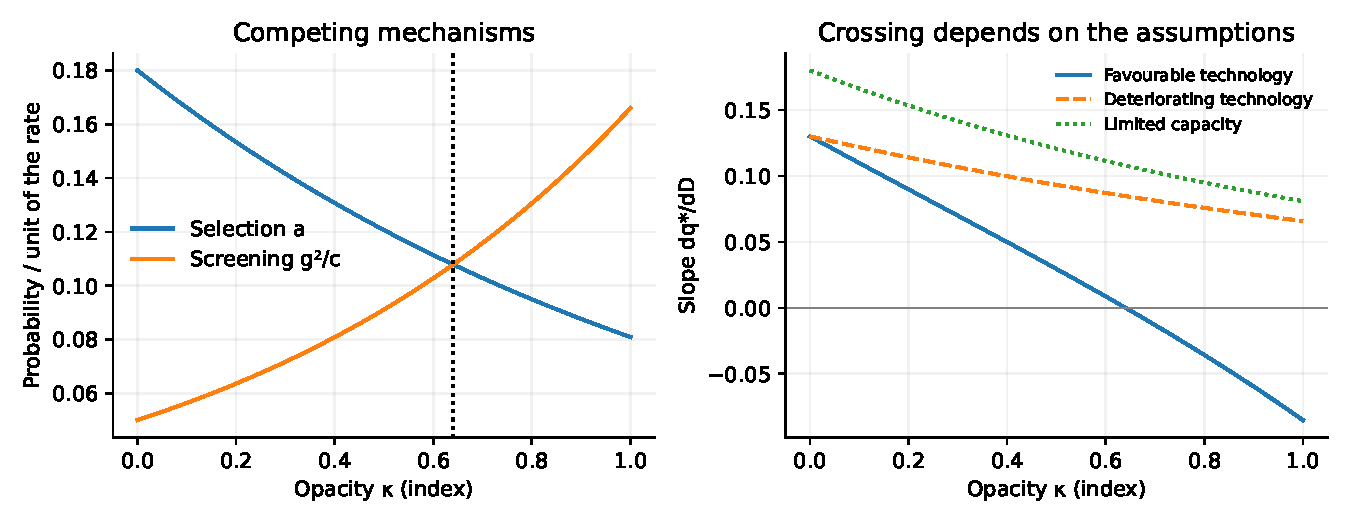
\includegraphics[width=\linewidth]{../code/figures/mechanisms_en.pdf}
\caption{Selection, screening, and crossing assumptions. The alternative
technology uses $g=\sqrt{0.05}e^{-0.4\kappa}$ while cost continues to increase.
Limited capacity is $\bar e=0.08$. Source: illustrative simulations,
\texttt{code/verify.py}. Slopes are measured per unit of the decimal rate.}
\label{fig:mechanisms}
\end{figure}

Figure~\ref{fig:mechanisms} includes an equally admissible scenario in which
$g$ declines, giving $H=0.05e^{-1.2\kappa}$. Then
$a/H=3.6e^{0.4\kappa}>1$ throughout the interval, so there is no reversal.
The code also shows that capacity of $0.08$ keeps the risk slope positive
even with favourable screening technology. Both examples contradict an
unconditional interpretation that opacity reverses the sign.

\subsection{Corners and numerical stability}
Figure~\ref{fig:corners} uses two additional configurations. With
$\bar q=0.35$, $a=0.04$, $g=0.4$, $c=1$, and $\bar e=0.44$, capacity
begins to bind at $D=0$. To the left, the risk slope is
$0.04-0.16=-0.12$; to the right, it is $0.04$. The solution is continuous
but not differentiable at that point. In the second configuration,
$\bar q=0.04$, $a=0.04$, $g=0.5$, $c=1$, and $\bar e=1$ lead to the
risk floor, which stops further reductions. The unconstrained first-order
condition would imply negative probabilities and hence an invalid solution.

\begin{figure}[htbp]
\centering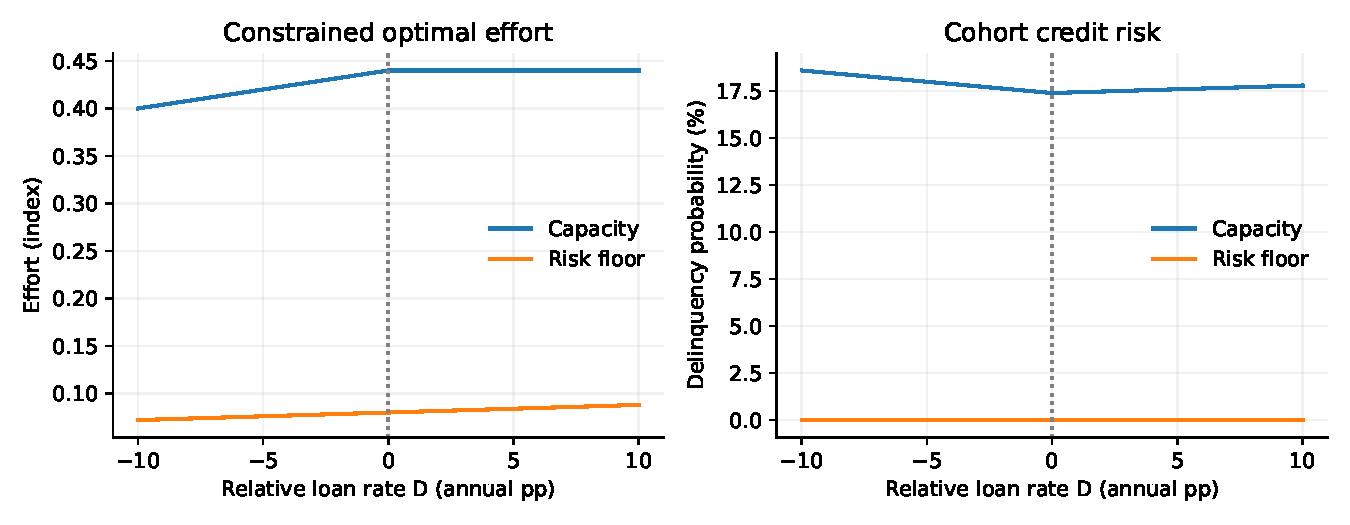
\includegraphics[width=.95\linewidth]{../code/figures/corners_en.pdf}
\caption{Effort and risk with capacity and a probability floor. $D$ is in
annual percentage points and risk in per cent. Source:
\texttt{code/verify.py}, hypothetical parameters. The zero floor is a
boundary of the linear technology, not a policy recommendation.}
\label{fig:corners}
\end{figure}

The analytical solution is compared with a bounded SciPy optimiser that
evaluates the objective directly and includes both endpoints as candidates.
Of 1500 draws with seed 20261110, 1495 are admissible: 765 interior, 293
capacity-constrained, and 437 at the risk floor. The maximum effort difference
is below $4\times10^{-8}$, against a required tolerance of $2\times10^{-6}$.
Slopes are checked with central differences of step $10^{-6}$ only when all
three points remain in the same regime; the maximum error is below
$1.1\times10^{-10}$. Zero capacity is checked, and invalid probabilities,
zero cost, negative productivity, and nonpositive payoffs are rejected.
Required checks raise exceptions on failure, so they remain active when
Python runs with optimisation enabled.

\subsection{A composition counterexample}
At $\kappa=0$ and $D=0$, interior screening gives $q^*=0.225$ and
$\beta_D=\cohortSlope$. Set $B_0=4$, $B_1=1$, $m_0=0.10$, and
$\varepsilon=3$. Then $w=0.2$ and
\[
M'=0.2[0.13-3(0.8)(0.225-0.10)]=\stockSlope<0.
\]
All probabilities and balances are valid. A one-percentage-point rate
increase has a local new-risk response of $0.13$ percentage points but a
total-ratio response of $-0.034$ percentage points. These are local
derivatives, not the effects of a large discrete change or causal estimates.

\begin{figure}[htbp]
\centering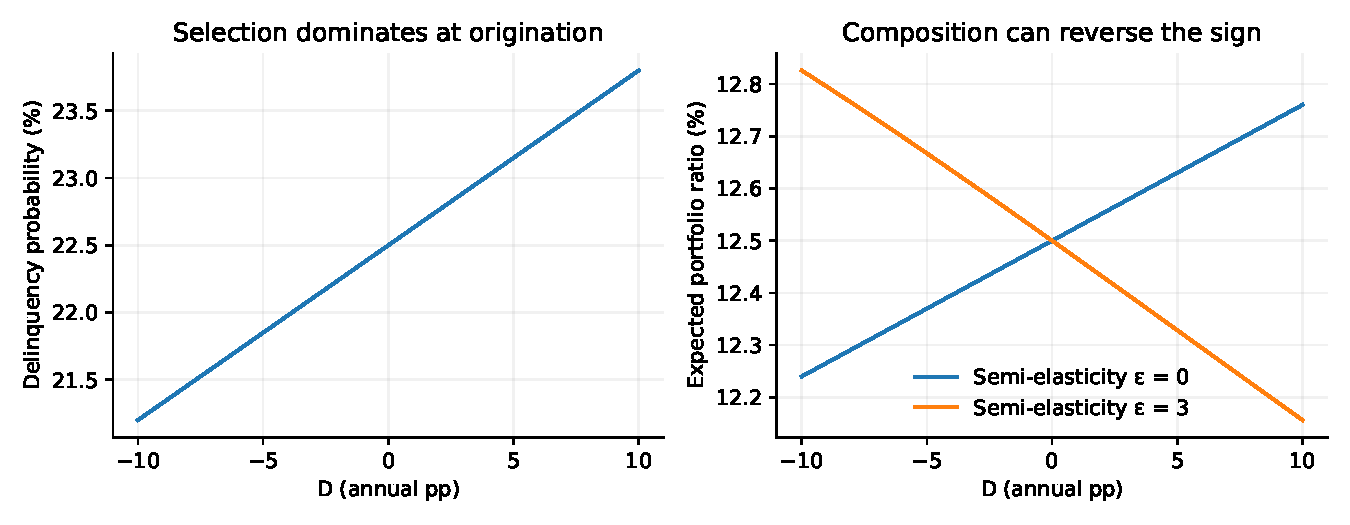
\includegraphics[width=\linewidth]{../code/figures/stock_composition_en.pdf}
\caption{The same cohort risk can accompany opposite portfolio slopes.
With a fixed weight ($\varepsilon=0$), the sign is transmitted. With a
sensitive balance ($\varepsilon=3$), composition dominates. Source:
illustrative simulations, \texttt{code/verify.py}.}\label{fig:stock}
\end{figure}

P3 also identifies the required magnitude of the balance response. At the
counterexample point, $\beta_D=0.13$ and $q^*-m_0=0.125$. For each
$0<w<1$,
\[
M'<0\quad\Longleftrightarrow\quad
\varepsilon>\frac{0.13}{(1-w)0.125}=\frac{1.04}{1-w}.
\]
At $w=0.20$, the cutoff is $1.3$: quality dominates below it, the two effects
cancel at equality, and composition dominates above it. The value
$\varepsilon=3$ lies in the last region. Figure~\ref{fig:frontier} displays
the same inequality for different balance ratios, holding risk and its
slope at the comparison point fixed. These regions are not observed bank
frequencies.

\begin{figure}[htbp]
\centering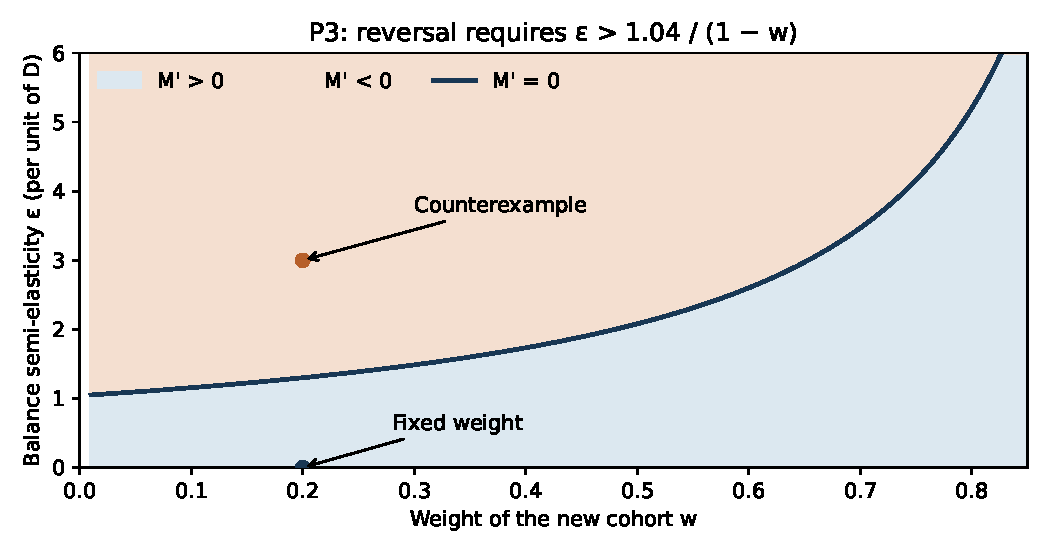
\includegraphics[width=.82\linewidth]{../code/figures/composition_frontier_en.pdf}
\caption{P3 sign-reversal frontier at $D=0$, with $\beta_D=0.13$ and
$q^*-m_0=0.125$. Each weight corresponds to a different ratio of positive
balances, held fixed when differentiating. The line gives $M'=0$; above it
$M'<0$, and below it $M'>0$, for $0<w<1$. Source:
\texttt{code/reader\_checks.py}, called by \texttt{code/verify.py}.
The figure implements the same illustrative P3 inequality.}\label{fig:frontier}
\end{figure}

Proposition~\ref{p:stock} is checked at 51 opacity values, 25 prices, and
four values of $\varepsilon$, always where derivatives are well-defined.
The maximum difference from finite differences is below $3\times10^{-11}$.
SymPy separately checks the product rule and the derivative of the exponential
weight. This double check reduces the risk of repeating an error in both a
formula and its implementation, without replacing the general proof.

Verification contains 4018 baseline checks and 73 additional checks of
reference probabilities, admissible primitives, balances and their derivatives,
rational arithmetic, and signs on either side of the frontier at seventeen
weights. Additional results are recorded in
\path{code/output/reader_verification.json}. These checks can detect
implementation errors in the cases examined; general validity rests on the
proofs.

\begin{figure}[htbp]
\centering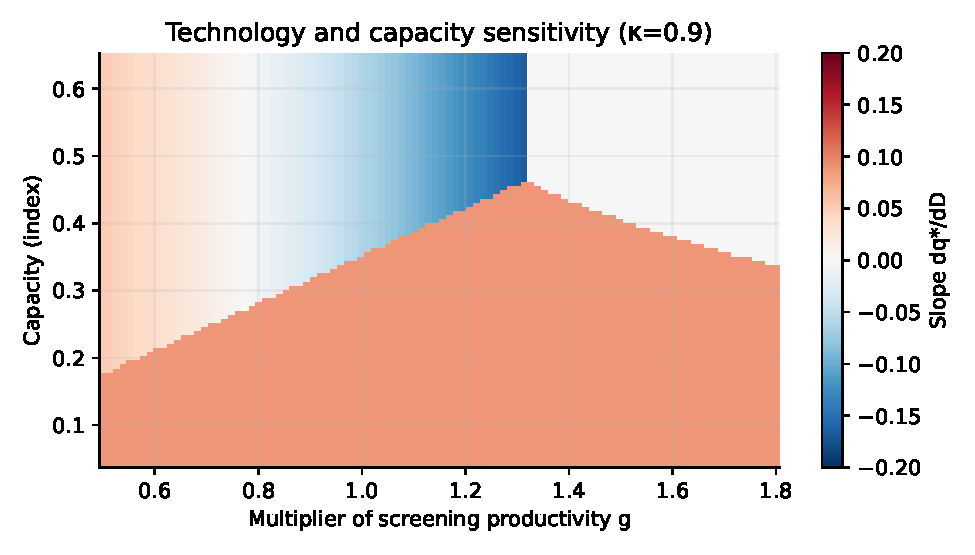
\includegraphics[width=.80\linewidth]{../code/figures/sensitivity_en.pdf}
\caption{Sensitivity of the slope to productivity and capacity at
$\kappa=0.9$. The map includes the effective regimes and the probability
floor, rather than extrapolating an interior condition outside its domain.
Source: \texttt{code/verify.py}, hypothetical simulation.}\label{fig:sensitivity}
\end{figure}

Figure~\ref{fig:sensitivity} varies capacity and productivity, holding the
remaining parameters fixed. Higher productivity does not generate an
unboundedly negative slope: saturation at zero risk makes the slope zero.
The exercise identifies regions of the model, not their frequency among
Peruvian banks. Without screening information, a bank cannot be assigned
to a region from its observed rate alone.

\section{Discussion and Empirical Implications}
\subsection{Comparative statics, prediction, and causality}
The derivative $\partial_Dq^*$ compares screening problems at nearby prices:
it holds primitives fixed and allows effort to adjust optimally. It is
therefore a conditional comparative static. A predictive coefficient of
$M_{t+h}$ on $D_t$, by contrast, summarises a joint distribution of prices,
technology, composition, and shocks. A causal effect of changing price
additionally requires identification of an intervention and modelling of
demand and peer responses. These are distinct objects even when they use
the same observable variables.

Pricing lies outside the continuation problem. The model consequently
characterises the screening response to a given price but does not determine
the equilibrium price. This scope isolates the mechanism without giving the
result a causal interpretation, a rate-setting recommendation, or the status
of an optimal supervisory rule.

\subsection{Requirements for evaluating predictive content}
An empirical evaluation consistent with the model requires a bank-month
panel, comparable rates by cell, lagged balance weights, and documented
coverage. A twelve-month horizon allows subsequent performance to be studied,
provided the credit event is defined consistently. For example, loans more
than ninety days past due must be treated as a separate target from the
accounting delinquency ratio when their definitions differ.

The relevant comparison is between a forecast based on lagged delinquency
and the economic cycle and its extension with relative loan pricing. The
own spread, defined as the bank rate minus a reference, must be distinguished
from the mean peer spread defined using the same reference. Since $D$ is
their difference, including all three regressors creates exact collinearity.
The forecasting specification must respect that identity.

Information timing is equally important. At forecast origin $t$, training
can only include observations whose outcome at $t+h$ has already been
published. Unknown outcomes must therefore be purged from the end of the
training window. Weights, scales, missing-data treatment, and comparability
rules must be estimated from past information and fixed before evaluation.
If historical series have been revised and archived vintages are unavailable,
the exercise is a pseudo-real-time evaluation.

Both forecasts must be evaluated on the same banks and dates. Cross-bank
dependence and overlapping errors at long horizons require explicit
inferential treatment. The Clark--West test is an option for nested models
under its conditions. Lower forecast error is an empirical result to be
measured, not a consequence of the propositions. Likewise, an undetected
improvement may reflect measurement error, low power, or regime changes as
well as the information actually contained in prices.

\subsection{Assumptions that bound interpretation}
Reduced-form selection and linear technology make the mechanism transparent
but restrict its scope. Effort does not change lending volume, and neither
applicants nor peers act strategically within the model. The opacity index
does not itself provide an empirical segment classification. P2 crossing
requires S4; without those conditions, opacity can vary without reversing
the slope.

The P3 bridge also requires compatible events, horizons, and balances.
Write-offs, cures, portfolio sales, collateral, or currency exposure can
alter the relationship between new-loan risk and the total ratio.
Deterministic balances exclude the covariances associated with a random
denominator. Subtracting peer rates or including fixed effects cannot
substitute for these accounting assumptions.

These restrictions guide application. Distinguishing quality from composition
requires vintages and weights; attributing a response to screening requires
information on effort or its technology. Recoveries, concave screening,
or imperfect information at the bank would expand the problem but require
the optimum and transmission conditions to be derived again.

\section{Conclusions}
The informational content of relative loan pricing depends on the dominant
mechanism and the risk measure observed. The global screening solution shows
that selection minus screening determines the slope only at an interior
solution. Capacity and the probability floor change that rule even when
screening productivity is high. The opacity threshold requires continuity,
strict decrease, crossing, and interiority; it is not an automatic consequence
of opacity.

Moving from a cohort to the total outstanding balance introduces a second
margin: portfolio composition. The derivative of the ratio adds a changing-weight
effect to the quality effect, and the former can dominate and reverse the
sign. A fall in aggregate delinquency therefore need not mean that new-loan
risk has improved.

For Peruvian bank supervision, the result specifies how a rate gap should
be interpreted and tested: alongside screening capacity, loan vintages,
and portfolio turnover. The proofs and reproducible exercises establish
the mechanism's conditions. Measuring its predictive improvement requires
an empirical evaluation that respects definitions and the information
available at each date.\label{body:end}
\clearpage
\bibliographystyle{plainnat}\bibliography{references_en}
\clearpage\appendix

\section{Reproducibility and Supplementary Materials}
Complete proofs appear in the main text. Supplementary algebra is organised
in \path{hand/guia_derivaciones.tex}. The guide records manipulations,
rules, conditions, and units. It is typeset supporting material, not evidence
of a personal handwritten review. That distinction is made explicitly in
\path{hand/README.md}.

The single computational entry point, from the repository root, is:
\begin{verbatim}
python -m pip install -r code/requirements.txt
python code/verify.py
\end{verbatim}
It regenerates the six figures in Spanish and English, the files
\path{verification.json} and \path{reader_verification.json}, and the
numerical macros used in the article. Dependencies and the random seed are
pinned. The simulations require neither credentials nor network access;
\path{code/data/README.md} documents the source, units, and population of
the BCRP transcription. Topic-presentation materials are retained and
identified as historical documents.

\section{Lean Formalisation of the Propositions}\label{app:lean}
All three propositions have transparent specifications and general proofs
in Lean 4.30.0-rc2. Formalisation uses AppliedModelingLib and the course-required
configuration \path{gpt-5.6-sol}, reasoning effort \path{xhigh}. Checks run
on Linux with the unmodified official engine.

\begin{center}\small
\begin{tabular}{L{.06\linewidth}L{.21\linewidth}L{.15\linewidth}L{.47\linewidth}}
\toprule P. & Declaration & Status & Assumptions and coverage\\\midrule
P1 & \path{proposition1} & Proved & S1--S3: unique maximum, formulas, bounds, regimes, zero capacity, continuity, and one-sided derivatives.\\
P2 & \path{proposition2} & Proved & S1--S4: unique interior threshold and signs of the derivative.\\
P3 & \path{proposition3} & Proved & S1--S3 and S5: identity, derivative, sign preservation and reversal.\\
\bottomrule\end{tabular}
\end{center}
The namespace is \path{Galarza26RelativeCredit}. The files are:
\begin{itemize}
\item Proof declarations: \path{lean/ProofInterface.lean}.
\item Transparent specifications: \path{lean/PaperInterface.lean},
with suffix \texttt{Spec}.
\end{itemize}
Each declaration proves the exact type of its specification.
No additional mathematical hypotheses are introduced and no \texttt{sorry}
is used. The axiom closure of all three endpoints contains only
\texttt{propext}, \texttt{Classical.choice}, and \texttt{Quot.sound}.

The exact audited PDF, its commit, the official check result, and the evidence
graph are identified in
\href{https://github.com/fgalarzac/ai-project/blob/main/docs/lean_progreso.md}{\path{docs/lean_progreso.md}}.
That record distinguishes proof compilation, correspondence with the text,
and protocol closeout. Keeping it external permits source pinning without
a circular reference to the source's own hash. The Spanish and English
editions express the same model and results; the record explicitly identifies
the source submitted to validation.

Formal verification establishes consequences of definitions and assumptions.
It does not certify that Peruvian banks satisfy S5 or identify causal effects
or predictive gains. It also does not replace personal checking of the
derivations.

\clearpage
\section{Collaboration with Artificial Intelligence}
The \path{prompts.md} record preserves available verbatim interactions and
distinguishes summaries from original text. The table documents relevant
claims, the verdict applied, and the supporting check. These computational
checks are not attributed to an undocumented handwritten review by the author.

\begin{longtable}{L{.29\linewidth}L{.29\linewidth}L{.33\linewidth}}
\toprule Claim or contribution & Verdict and rationale & Check\\\midrule
\endhead
The two-stage problem is solved. &
Incomplete: price is given; optimisation concerns effort. &
Definition of the continuation problem and the global P1 proof.\\
The slope $a-g^2/c$ applies at every price. &
False outside the interior: capacity gives slope $a$ and the floor gives zero. &
P1, an independent optimiser, and the capacity example.\\
Opacity necessarily improves screening. &
Not a general implication: $2g'/g-c'/c$ may be negative. &
Identity \eqref{eq:logs} and the no-crossing scenario.\\
The new-risk sign carries over to the outstanding balance. &
Conditional: weights and legacy risk must satisfy the P3 restrictions. &
Composition identity and counterexample with $M'=-0.034$ and $q^{*\prime}=0.13$.\\
Subtracting peers removes all common exposure. &
Excessive: the additive base cancels, but heterogeneous loadings can remain. &
Decomposition with coefficients $\lambda_j$.\\
Figures in the thesis plan are replicated estimates. &
Excluded from empirical analysis because the materials do not provide a consolidated reproducible dataset. &
Separation of documented public statistics and illustrative parameters.\\
Simulations prove the general results. &
False: they check implementations and can detect errors in the cases examined. &
Complete proofs, independent checks, and Lean proofs.\\
One percentage point of price changes prior risk by $0.01a$ units. &
Correct: this is $a$ percentage points of risk. &
Unit conversion in S1 and the example with $a=0.18$.\\
\bottomrule
\end{longtable}

\section{Availability of Materials}
LaTeX sources, both language editions, figures, code, and formalisation
artifacts are distributed in the public repository cited on the first page.
\path{docs/fuentes.md} details the provenance and verification scope of each
source. Proposal and presentation documents retain their original dates and
definitions; this article identifies the specification used in its final
results.
\end{document}
